\chapter{Fundamentals}
\label{chap:funds}


To understand the design and implementations presented in the thesis, we first have to understand the connection between the different partaking modules \emph{NestKernel}, \emph{PyNEST}, and \emph{PyNESTML}. As these three modules are only used in orchestration if we build custom neuron and synapse models, this chapter will focus on the execution of simulation scripts that are using user defined external models. If multiple models are to be generated, PyNEST does not enforce the order of commands, as long as instances of models are not used prior to their generation in the script. Thus, to keep everything simple and consistent, the simulation script in the following description will always start by generating \emph{all} models \emph{collectively} and then installing them.

\section{NestKernel: the simulation backend}

This section serves as a basic introduction to the most important functionalities of NEST's simulation kernel, especially those that will be affected by the new implementation in \Autoref{chap:vec}. Registering new custom models and creating instances of them are the first steps in each simulation script, and usually the user does not have to worry about how instances are created. Once a model is registered, the NestKernel creates a \emph{factory} object responsible for creatins instances of the model and managing the modifications made to the attributes of the model by the user during the simulation . To further understand the role of the factory in the registration and creation of nodes, we have to take a deeper look at the source code and inspect the steps required in executing the simulation. In the subsequent section, we review the logic behind registering models and explain how to create node instances from these models.

In the introduction, we have already mentioned that PyNEST is the Python interface for NEST, executing NestKernel functions. Although this is conceptually true, the full picture is a bit more complicated in that each function call in PyNEST is (more or less directly) forwarded to NEST's simulation language interpreter \emph{SLI} \citep{gewaltig2007nest}. SLI is a stack-based language derived from PostScript \citep{adobe1990postscript} and outside the scope of the thesis. Figure \ref{fig:layer} depicts the three layers that are responsible for running a simulation, from the Python interface at the top to the C++ layer at the bottom. PyNEST takes the arguments from the simulation script and pre-processes the arguments for the SLI interface functions by converting them from Python to C++ objects and bringing them into a suitable form. SLI then calls the functions exposed by the NestKernel.

\begin{figure}[h!]
\centering
\includegraphics[width=0.5\textwidth]{src/pic/layers.png}
\caption{\textbf{\emph{NEST} layers}: At the top level, we have the user simulation script that imports the PyNEST module. The PyNEST functions represent an intermediate layer between the simulation script and the NestKernel. They prepare the arguments of the command and push them onto the stack in SLI. SLI retrieves the command and the arguments from the stack and calls the corresponding function in the NestKernel. The result then takes the same path in the reverse direction from the NestKernel to the simulation script. After the completion of the command in the context of the NestKernel, the results are pushed onto the stack, and SLI removes them from the stack and makes them available to the simulation script.}
\label{fig:layer}
\end{figure}

\subsection{Registering new models}

As an abstraction, we use \texttt{N} as a custom model that will be registered and show the order of operations in the message sequence diagram in the \autoref{fig:nestkernel_register}. Every custom model generated by \emph{NESTML} is shipped with two main components (see \autoref{fig:sli_install}). The first component is the implementation of the model itself in C++, the second is a class derived from \texttt{SLIModule}, which is responsible for registering the model in the NestKernel. By calling PyNEST's \texttt{Install()} function with the model library name as parameter, SLI searches for the library in the provided paths and dynamically loads it. Upon loading, SLI calls the \texttt{init()} function in the derived \texttt{SLIModule} class. The \texttt{SLIModule} instance calls \texttt{register\_node\_model()} in the NestKernel's \texttt{ModelManager} class. The function requires mainly two arguments: the class type name of the model as a \emph{template argument} and the name under which the model will be available to the user from SLI and PyNEST.

The function \texttt{register\_node\_model()} checks if another model under the same name already exists, and only proceeds to registering the model if its name is unique. Afterwards, a new instance of the \texttt{GenericModel<T>} class is created with our model \texttt{N} as the substituted type (i.e., \texttt{T = N}). The \texttt{GenericModel} class works as a factory, which is responsible for creating instances of \texttt{N}, which means that the user can not explicitly call the constructor of \texttt{N} and each creation of \texttt{N} is mediated by the \texttt{GenericModel}. Finally, the \texttt{ModelManager} regains control, sets the model parameters (for example the node instance's \emph{ID}) and lastly creates one \texttt{proxy} object of the model for each \emph{thread}. The \texttt{proxy} nodes are required for representing nodes residing in remote processes and allow for better performance during connection setup and event delivery in the simulation phase by avoiding remote lookups via the message passing interface. Finally, the \texttt{register\_node\_model()} returns the ID of the model to the \texttt{SLIModule} in its \texttt{init()} method. Inside the \texttt{init} method, we can also register other models by calling the \texttt{register\_node\_model()} on each model and inspect the values of the returned IDs.

\begin{figure}[ht!]
\centering
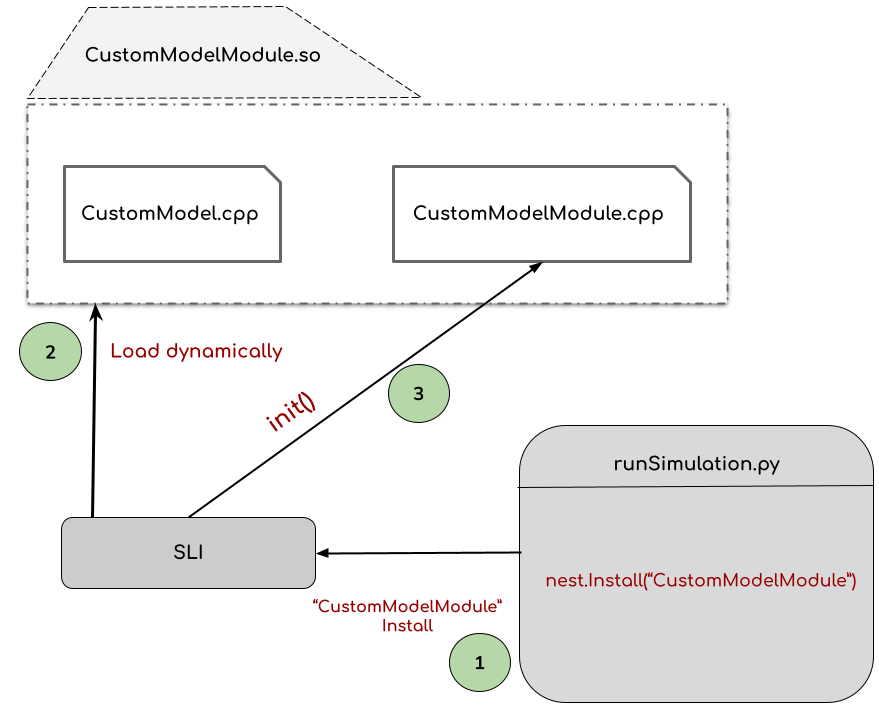
\includegraphics[width=0.7\textwidth]{src/pic/install_command.png}
\caption{\textbf{Installing an external module}: Each generated model comes with two main C++ files. The first is implementing the model's logic and functionalities, the second is for registering the model in the NestKernel. The process always starts at the simulation script level, the call to \texttt{Install()} in PyNEST gets the library name as an argument and starts the process of registering the model. The function pushes the command name and the library onto the SLI stack. SLI loads the library and creates an instance of the \texttt{SLIModule} representing the loaded module. The module then initiates the call to the \texttt{init()} function that starts the registration workflow for the new model in the NestKernel.}
\label{fig:sli_install}
\end{figure}

\vspace{0.5cm}
\begin{figure}[ht!]
\centering
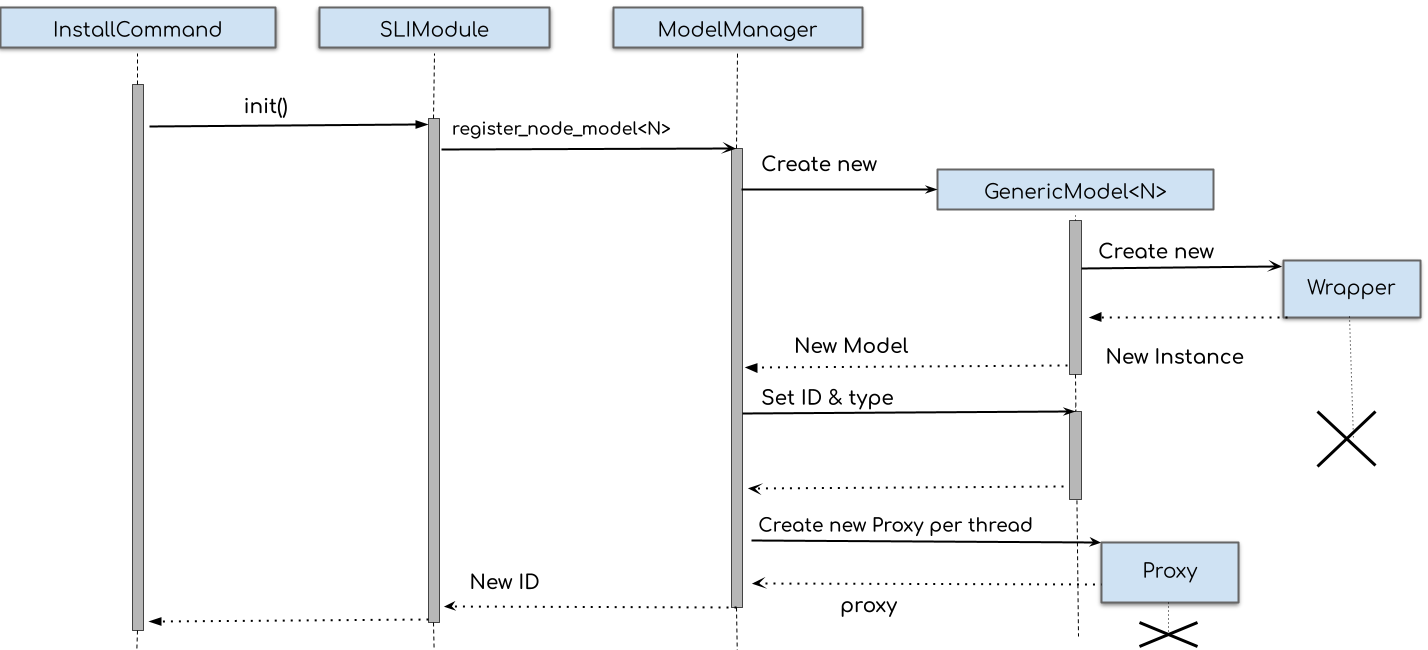
\includegraphics[width=\textwidth]{src/pic/register.png}
\caption{Registering new models in the NestKernel: The message sequence chart depicts the interaction between the components in the NestKernel responsible for registering new custom external models.}
\label{fig:nestkernel_register}
\end{figure}

\subsection{Creating new nodes}

The \texttt{NodeManager} is responsible for creating nodes, parametrizing them and handling their distribution over the available \emph{threads}. It is important to keep in mind that each node is exactly assigned to one thread, each thread can only modify its own nodes and non-local nodes are represented by \emph{proxies}. In addition, each thread knows the total number of nodes it has created. The second component for creating new nodes is the \texttt{GenericModel}, and as we have already mentioned in the previous subsection it plays the role of a \emph{factory} responsible for creating the real instances of the registered model. Each registered model \texttt{N} provides an implementation for \emph{cloning} that is required of creating new nodes. Upon requesting the creation of $n$ nodes, the \texttt{NodeMananger} calls the \texttt{GenericModel} to create an instance of the registered model, which creates a new empty copy of the model and returns it to the \texttt{NodeManager}. \autoref{fig:nestkernel_creation} depicts the steps involved in creating a new node.

\begin{figure}[ht!]
\centering
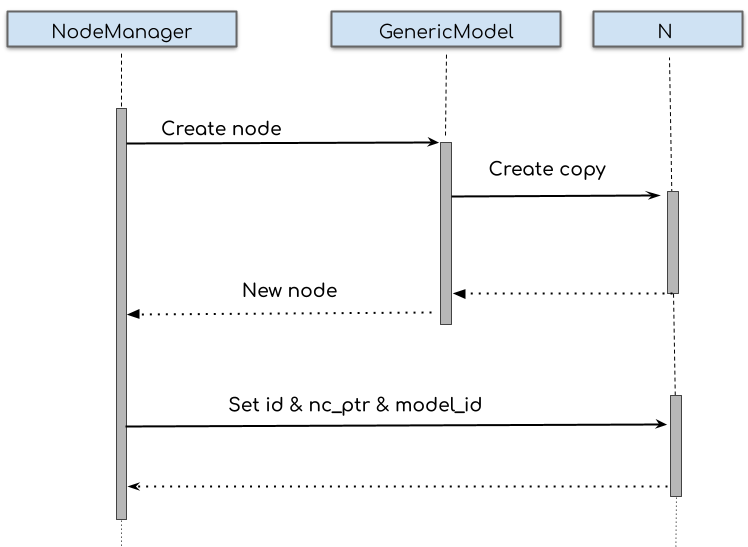
\includegraphics[width=0.6\textwidth]{src/pic/nodes_creation.png}
\caption{Creating new instances of the registered models in the NestKernel: The message sequence chart depicts the interaction between the components in the NestKernel responsible for creating new instances of any arbitrary registered model.}
\label{fig:nestkernel_creation}
\end{figure}

\section{PyNEST: the simulation frontend}

Although PyNEST and the NestKernel are usually used together, they are completely separated and independent modules. As explained above, the only way for the both of them to communicate is through the \emph{SLI} interface. As shown in \autoref{fig:pynest} (taken from \citep{epp}), PyNEST is split into two layers. The \emph{low-level API} is responsible for ensuring the smooth communication between Python and SLI by providing the necessary functionalities for converting data from SLI to Python and back. The \emph{low-level API} is based on a Python extension created using Cython. It only uses three functions to communicate with \emph{SLI}: The \texttt{sli\_push()} function for pushing function arguments and other data to the operand stack of SLI, \texttt{sli\_pop()} for retrieving (return) values from the stack and \texttt{sli\_run()} for executing commands. The functions \texttt{sli\_push()} and \texttt{sli\_pop()} are also responsible for converting the data (arguments and results) between the interfaces.


\begin{figure}[ht!]
\centering
\includegraphics[width=0.7\textwidth]{src/pic/The-architecture-of-PyNEST-The-lowest-level-is-the-simulation-engine-It-is-used-by.png}
\caption{The architecture of PyNEST (taken from \citep{epp}): The lowest level is the simulation engine implemented by the NestKernel. It is used by the simulation language interpreter SLI and by the PyNEST low-level API. The PyNEST high-level API uses the low-level API to communicate with the simulation engine. The user’s simulation code can use functions from PyNEST, from Python, and from its extension modules.}
\label{fig:pynest}
\end{figure}

As using only the three low-level API functions of PyNEST is not very convenient and might not be very intuitive for non-programmers, the high-level API provides all necessary functions for creating the network and running simulations directly by providing wrappers around common SLI commands. It covers all main functionalities in SLI and uses the low-level API for data transfer and code execution. Simulation scripts are usually based on the high-level API functions.

The \texttt{Create()} function is responsible for creating new instances of registered models. It takes four parameters: the model name, the number of instances, the parameter values for the new nodes and a spatial distribution of the nodes. Only the model name is a required parameter, all the others are optional. Omitting the number of instances, the \texttt{Create} function creates a single instance. Discarding the model parameters, the created node(s) will be instantiated with default values and the nodes will not have any spatial information if the spatial parameter is omitted. The return value of the function is a \texttt{NodeCollection} object, which is a compact representation of the nodes in the NestKernel. All functions that handle nodes in PyNEST expect \texttt{NodeCollection} objects to identify the nodes to operate on. An important feature of the \texttt{NodeCollection} class is that it only stores a contiguous set of nodes. Thus, creating many nodes only requires storing the position of the first and the last position of the nodes in the list, instead of a full list. Since the class is also \emph{iterable}, it supports indexing, splitting and concatenating as if all node identifiers were present.

The \texttt{NodeCollection} allows retrieving values from the created nodes by calling the \texttt{get()} function. Depending on the number of provided keys, the \texttt{get} function either returns a \emph{list} or \emph{dictionary} containing the values of the given keys. We can also change the values of the contained nodes by calling the \texttt{set()} function. Setting is generally a bit more complicated, as the given value might have different interpretations in the NestKernel depending on the number of the nodes in the \texttt{NodeCollection} and the type of value (\emph{single value} versus \emph{list}). In general, it is possible to set the parameters of a single node or multiple nodes with a single function call.

Another important feature in PyNEST is copying models. After registration, the NestKernel allows users to copy existing models, parametrize them differently and assign them a new name. The function responsible for copying the models is called \texttt{CopyModel()}.

A network can be created from node instances by calling the \texttt{Connect()} function. It takes two \texttt{NodeCollection} objects, the first being treated as the \emph{pre-synaptic} (or \emph{source}) population, the second being the \emph{post-synaptic} (\emph{target}) population. By supplying extra parameters, the type of the connection and a \emph{connection rule} can be specified. Connection rules in this context are defining the connection pattern, like \emph{fixed indegree}, \emph{all-to-all} or \emph{pairwise Bernoulli}.

To simulate the created network for a given amount of time, we have the \texttt{Simulate()} function with the time $t$ as a parameter. It simulates the created network for $t$ milliseconds.

The PyNEST high-level API obviously provides many other important functions, like those for inspecting the topology of the created network, changing the number of working threads and configuring the NestKernel itself. However, as we are mainly interested in the functions related to the topic of this thesis, we restrict the desctiption here to the functions mentioned above and introduce other functions in later chapters if they are needed for understanding a concept presented there.

\section{PyNESTML: the code generator}

As explained in \autoref{chap:intro}, models for NEST are created using the NEST Modelling language NESTML. To make its use easier for the users, NESTML also provides a convenient Python interface called PyNESTML. For simplicity, we sometimes use the terms NESTML and PyNESTML interchangibly.

The first step in each simulation script using an external model is to call the \texttt{generate\_target()} function that is responsible for all steps to make the model available to the NestKernel. This includes generating the code, building the library and adding it to the installation path. The function takes a set of mandatory parameters to ensure the correctness of the code generation. The first parameter is the \texttt{input\_path} which specifies the location of the model in the file system. If this parameter is given as a list of paths, NESTML will generate the code for multiple models at once. In this thesis we only use the second form when we want to co-generate neuron and synapse models together, and in all other cases we only generate one model at a time.

The second important parameter is the dictionary \texttt{codegen\_opts} which is responsible for providing extra information about the neuron and the logic for creating the library code. Most importantly, this parameter can contain a specification of (\emph{neuron}, \emph{synapse}) pairs that PyNESTML needs to co-generate. In this case, the synapse model is bound to the listed \texttt{neuron} model and vice versa.

PyNESTML can generate code for different target platforms, but for the scope of the thesis, we focus on NEST as the \texttt{target\_platform}. In the scope of the thesis, the remaining parameters are not of importance and do not affect the execution flow. We will thus omit them in all following descriptions.

\begin{figure}[ht!]
    \centering
    \includegraphics[width=0.9\linewidth]{src/pic//nestml_model.png}
    \caption{\textbf{The neuron NESTML model \cite[taken from][]{perun2018reengineering}}: A neuron in NESTML is always declared with the \emph{neuron} keyword with providing the name that will be used to uniquely identify the model in the simulation. Each neuron may have several blocks defining its behave during the simulation. The \emph{state}, \emph{parameters} blocks hold the model's attributes that can be set before running the simulation. The attributes inside the parameters blocks are invariant during the simulation. The attrbiutes in the state block however are subject to change. The manner how the attributes in the state block may change is defined in the \emph{update} block. The update block defines how the neuron model should behave during each step in the simulation. The in- and out-ports of the neuron are defined in the input and output block. A model written in NESTML can be configured to
    receive two distinct types of input: spikes and continuous-time values.} 
    \label{fig:neuron_model}
\end{figure}


A neuron model in NESTML is composed of different blocks and it is depicted in \autoref{fig:neuron_model}. The \texttt{state} block defines a set of state variables and their initial values upon instantiation. These are updated by the equations during the simulation. The \texttt{parameters} block declares a set of variables that are not affected by the model equations and can be considered constants from the simulator point of view, but can be set by the user. The \texttt{internals} block behaves like the \texttt{parameters} block with the only difference that its variables can not be set by the user and their initialization expression can only reference parameters or other internal variables. The \texttt{equations} block specifies the \emph{differential equations} that describe the time evolution of variables in the \texttt{state} block. In the \texttt{update} block, users can describe the steps for updating the state of the neuron instance from one time step to the next during the simulation run and the \texttt{input} and \texttt{output} blocks define the types of the accepted incoming and outgoing signals, respectively. \vspace{1em}


The definition of a synapse model in NESTML is very similiar to defining the neuron model. The only two difference in writing a synapse model starts with giving the \emph{synapse} keyword in the NESTML model instead of the \emph{neuron} keyword. The second difference is in the \emph{update} block. The synapse model does not have an update block, but instead it has one or more \emph{onReceive} blocks, that are reponsbile for handling the event when an input spike is received by the synapse. Everthing else is the same as in the neuron model.

Each neuron model in NESTML is read by a parser and converted to an intermediate representation known as the abstract syntax tree (\emph{AST}). After parsing the model and making sure that the described model is syntactically correct, the generated intermediate representation in the form of the AST undergoes several transformations. Such transformations cover an analysis of the differential equations, processing of the \texttt{update} block and creating \emph{hooks} for solver code from the GNU Scientific Library. After applying these transformations, the AST goes through an optimization step, which includes \emph{constant folding} by eliminating expressions that calculate a value that can already be determined before code execution.

\autoref{fig:pynestml_workflow} summarizes the complete workflow of the code generation in PyNESTML. The process starts by feeding the \texttt{.nestml} file containing the model description to the code generator pipeline. A parsing and a validation step take place, where the model is checked for syntactic correctness and if it satisfies the code generator rules. Once the checks are complete, the pipeline moves to transforming the model into an intermediate representation in order to target different platforms. The third step is then the actual code generation, which is based on a set of templates written in \emph{Jinja} \citep{jinja} providing the implementation of the model in for the desired target platform. The last step in the pipeline controls the compilation and builds the model into a \emph{shared library} that can be loaded at runtime in the NestKernel using the \texttt{Install()} function in PyNEST.

\begin{figure}[ht!]
\centering
\includegraphics[width=0.8\textwidth]{src/pic/internal_workflow.png}
\caption{An overview of the processing workflow in PyNESTML: The process starts by feeding the NESTML models to the code generation pipeline. The first step in the pipeline starts by parsing the models and validating their syntax. Once the first step is completed, the models are transformed from NESTML files to AST objects. The pipeline moves to the next step by transforming the AST objects. The transformations may extend the structure of the AST by introducing new attributes or modifying model attributes. The last step in the pipeline takes the transformed AST object and generates the C++ code for the model by using custom defined templates. If all steps are completed without any failure, the pipeline can compile and build a library from the generated code of the model on request and make it available for the simulation.}
%\source{\url{https://nestml.readthedocs.io/en/latest}}
\label{fig:pynestml_workflow}
\end{figure}


